%%%%\%%%%%%%%%%%%%%%%%%%%%%%%%%%%%%%%%%%%%%%%%%%
%% Introduction aux Systèmes d'exploitation  %%
%%   * Historique                            %%
%%   * Principes fondamentaux                %%
%%   * Grandes classes de systèmes           %%
%%%%%%%%%%%%%%%%%%%%%%%%%%%%%%%%%%%%%%%%%%%%%%%

\title{Systèmes d'exploitation, 2ème année}
\subtitle{Multi-Threading}

\author{Yves \textsc{Stadler}}
\institute{Université de Lorraine - IUT de Metz}

\date{\today}

\begin{document}

%%
% Page de Titre
%%
\begin{frame}
\titlepage
\end{frame}

\def\sectitle{Agenda}
\section{\sectitle}
\def\subsectitle{Plan du cours}
\subsection{\subsectitle}
\begin{frame}{\sectitle}
    \begin{block}{\subsectitle}
        \begin{itemize}
            \item Différence entre Threads et Processus
            \item Utilisation des threads
            \item Synchronisation et ordonnancement
            \item Implémentation du multi-threading avec pthread
        \end{itemize}
    \end{block}
\end{frame}


\def\sectitle{Thread}
\subsection{\sectitle}
%%Frame
\begin{frame}{\sectitle}
    %%Block
    \def\subsectitle{Définition}
    \subsection{\subsectitle}
    \begin{exampleblock}{\subsectitle}
        \begin{itemize}
            \item Exécution de code en parallèle.
            \item Partage de données
            \item Être plus efficace que les processus (changement de contexte
                coûteux)
            \item Exploiter les capacités multi-processeurs.
        \end{itemize}
    \end{exampleblock}
\end{frame}

\def\sectitle{Différence entre Threads et Processus}
\section{\sectitle}
\begin{frame}{\sectitle}
    \def\subsectitle{Points communs}
    \subsection{\subsectitle}
    \begin{block}{\subsectitle}
        \begin{itemize}
            \item Permet d'obtenir plusieurs instructions s'exécutant en
                parallèle.
            \item Doivent se partager les ressources
        \end{itemize}
    \end{block}

    \def\subsectitle{Différences}
    \subsection{\subsectitle}
    \begin{block}{\subsectitle}
        \begin{itemize}
            \item Les threads sont comme des processus au niveau d'une
                application
            \item Les threads partages leur mémoire
            \item L'ordonnancement des threads peut être contrôlé
            \item Les changments de contextes sont plus efficaces
        \end{itemize}
    \end{block}
\end{frame}


\def\sectitle{Comportement du threads}
\subsection{\sectitle}
%%Frame
\begin{frame}{\sectitle}
    %%Block
    \def\subsectitle{Partage}
    \subsection{\subsectitle}
    \begin{block}{\subsectitle}
        \begin{itemize}
            \item Partage: du tas, des fonctions
            \item Pas de partage de la pile (mais accès possible!!)
            \item Partage du temps alloué au processus entre les threads 
        \end{itemize}
    \end{block}

    %%Block
    \def\subsectitle{Utilisation des piles}
    \subsection{\subsectitle}
    \begin{block}{\subsectitle}
        \begin{itemize}
            \item Une pile applicative
            \item Une pile système
            \item Un thread est toujours créer par un autre thread (allocation +
                appel système)
            \item Les threads se détruisent eux-même (pas de retour de l'appel,
                ne peut pas désallouer sa mémoire applicative)
        \end{itemize}
    \end{block}
\end{frame}

\def\sectitle{Thread et langages}
\subsection{\sectitle}
%%Frame
\begin{frame}{\sectitle}
    %%Block
    \def\subsectitle{Bibliothèques}
    \subsection{\subsectitle}
    \begin{block}{\subsectitle}
        \begin{itemize}
            \item ADA : type task
            \item Java : class Thread
            \item C, C++: pthread
        \end{itemize}
    \end{block}
\end{frame}

\def\sectitle{État des threads}
\subsection{\sectitle}
%%Frame
\begin{frame}{\sectitle}
    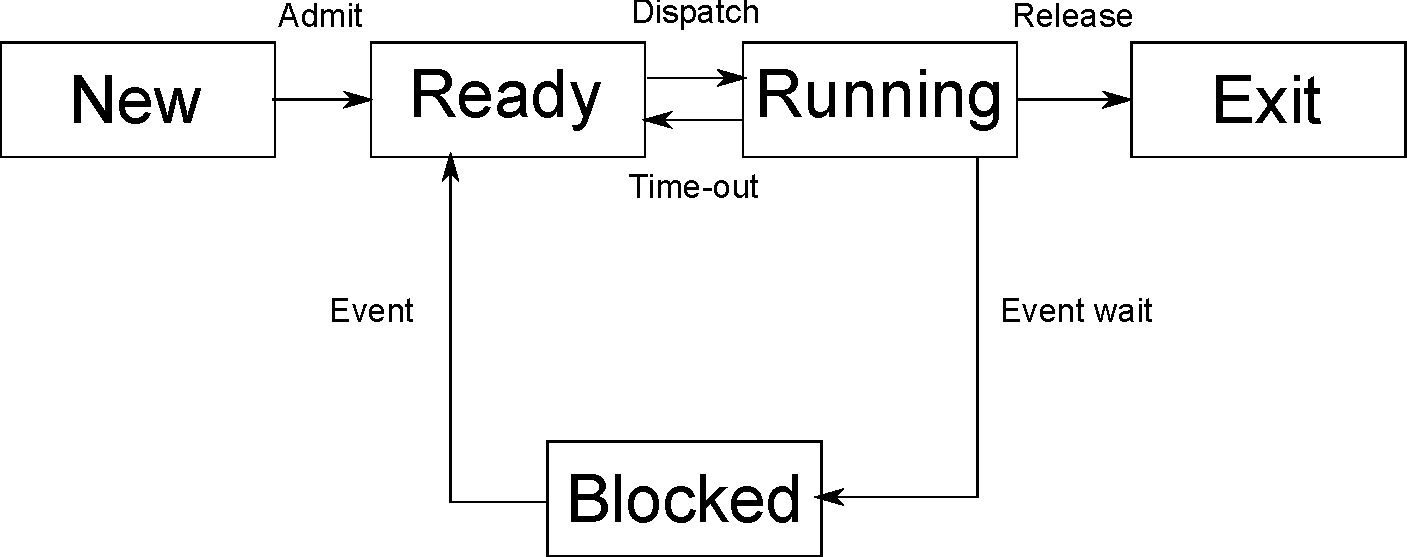
\includegraphics[width=\textwidth]{../images/StateSimple.pdf}
\end{frame}


\def\sectitle{Ordonnancement}
\subsection{\sectitle}
%%Frame
\begin{frame}{\sectitle}
%%Block
\def\subsectitle{Remarque}
\subsection{\subsectitle}
\begin{block}{\subsectitle}
\begin{itemize}
    \item Un processus choisi comment répartir son temps entre les threads qui
        le composent. 
\end{itemize}
\end{block}
%%Block
\def\subsectitle{Classe d'ordonancement}
\subsection{\subsectitle}
\begin{block}{\subsectitle}
\begin{itemize}
    \item Ancienneté (FIFO)
    \item Priorités (Fixes, variables)
    \item Quantum de temps durée max.
    \item Échéances
    \item Tourniquet
    \item Priorité et quantum
\end{itemize}
\end{block}
\end{frame}


\def\sectitle{User thread, Kernel thread}
\section{\sectitle}
%%Frame
\begin{frame}{\sectitle}
    \def\subsectitle{User thread}
    %%Block
    \subsection{\subsectitle}
    \begin{block}{\subsectitle}
        \begin{itemize}
            \item Géré par les librairies
            \item Le système n'en a pas conscience
            \item S'ordonnange entre eux.
            \item Ne peuvent pas de multi-threading
            \item Si un appel bloquant est fait par un thread, les autres sont
                bloqués.
        \end{itemize}
    \end{block}
    %%Block
    \def\subsectitle{Kernel thread}
    \subsection{\subsectitle}
    \begin{block}{\subsectitle}
        \begin{itemize}
            \item Au moins un thread kernel par processus.
            \item Reconnus par le systèmes qui gère leur ordonnancement.
        \end{itemize}
    \end{block}
\end{frame}


\def\sectitle{Modèles}
\section{\sectitle}
%%Frame
\begin{frame}{\sectitle}
    %%Block
    \def\subsectitle{One to one (1:1)}
    \subsection{\subsectitle}
    \begin{block}{\subsectitle}
        \begin{itemize}
            \item Les threads utilisateurs sont associés à une entité
                ordonnançable du kernel. (LWP)
            \item Win32, Linux, Solaris, NetBSD, FreeBSD
            \item double pile
        \end{itemize}
    \end{block}
    %%Block
    \def\subsectitle{Many to on (N:1)}
    \subsection{\subsectitle}
    \begin{block}{\subsectitle}
        \begin{itemize}
            \item Tous les threads utilisateurs d'un processus sont associés à
                un seul thread kernel.
            \item Pas de multi-threading
            \item On peut toujours éviter les appels systèmes pour éviter les
                bloquage (quand c'est possible)
            \item Implémentable sur des machines qui ne connaisse pas le
                threading.
            \item GNU Portable Threads
        \end{itemize}
    \end{block}
\end{frame}


\def\sectitle{}
\section{\sectitle}
%%Frame
\begin{frame}{\sectitle}
    %%Block
    \def\subsectitle{Many to manuy (M:N)}
    \subsection{\subsectitle}
    \begin{block}{\subsectitle}
        \begin{itemize}
            \item Sur certaines machines seulement
            \item Il faut ordonnancer les différents user-threads sur les kernel
                threads
            \item Assez complexe.
        \end{itemize}
    \end{block}
\end{frame}


\def\sectitle{Pthreads}
\section{\sectitle}
%%Frame
\begin{frame}[containsverbatim]{\sectitle}
    %%Block
    \def\subsectitle{Création / Destruction}
    \subsection{\subsectitle}
    \begin{block}{\subsectitle}
        \begin{itemize}
            \item type \verb+pthread_t+
            \item \verb+pthread_create(3)+ 
            \item \verb+pthread_t+, des attributs, la fonction de démarrage
                (pointeur)
            \item se termine en invoquant \verb+pthread_exit(3)+
            \item Un programme peut attendre la terminaison d'un trhead avec
                \verb+pthread_join(3)+
        \end{itemize}
    \end{block}


    %%Block
    \def\subsectitle{Mutex}
    \subsection{\subsectitle}
    \begin{block}{\subsectitle}
        \begin{itemize}
            \item \verb+pthread_mutex_t mutex1 = PTHREAD_MUTEX_INITIALIZER;+
            \item \verb+pthread_mutex_[un]lock+
        \end{itemize}
    \end{block}
\end{frame}


\def\sectitle{Attributs}
\subsection{\sectitle}
%%Frame
\begin{frame}[containsverbatim]{\sectitle}
    %%Block
    \def\subsectitle{Type}
    \subsection{\subsectitle}
    \begin{block}{\subsectitle}
        \begin{itemize}
            \item \verb+pthread_attr_t+
        \end{itemize}
    \end{block}
    %%Block
    \def\subsectitle{Ordonnancement}
    \subsection{\subsectitle}
    \begin{block}{\subsectitle}
        \begin{itemize}
            \item \verb+SCHED_FIFO+, FIFO, temps-réel
            \item \verb+SCHED_RR+, round-robin
            \item \verb+SCHED_OTHER+, ordinaire
        \end{itemize}
    \end{block}
    %%Block
    \def\subsectitle{Autres paramètres}
    \subsection{\subsectitle}
    \begin{block}{\subsectitle}
        \begin{itemize}
            \item Taille de la pille
            \item Taille de la zone de protection de la pile
            \item Joinable and detached
            \item Priorité
        \end{itemize}
    \end{block}
\end{frame}

\def\sectitle{Attention}
\section{\sectitle}
%%Frame
\begin{frame}[containsverbatim]{\sectitle}
    %%Block
    \def\subsectitle{Tread-safety}
    \subsection{\subsectitle}
    \begin{block}{\subsectitle}
        \begin{itemize}
            \item Les fonctions qui utilises des variables globales ne sont pas
                sûres
            \item Il faut user de mutex dans ce cas.
            \item De plus en plus de fonctions ont des équivalents "thread safe"
                (\verb+strtok+ et \verb+strtok_r+)
        \end{itemize}
    \end{block}
\end{frame}


\def\sectitle{Threads en Java}
\section{\sectitle}
%%Frame
\begin{frame}{\sectitle}
    %%Block
    \def\subsectitle{Dérivation de la classe Thread}
    \subsection{\subsectitle}
    \begin{block}{\subsectitle}
        \begin{itemize}
            \item Implémentation de la fonction run.
            \item Lancement avec la fonction start.
        \end{itemize}
    \end{block}

    %%Block
    \def\subsectitle{Implémentation de l'interface runnable}
    \subsection{\subsectitle}
    \begin{block}{\subsectitle}
        \begin{itemize}
            \item Implémenation de la fonction run
            \item Lancement avec la fonction start.
        \end{itemize}
    \end{block}
    %%Block
    \def\subsectitle{Pourquoi deux méthodes}
    \subsection{\subsectitle}
    \begin{block}{\subsectitle}
        \begin{itemize}
            \item Pas d'héritage multiple en java
            \item Applets 
        \end{itemize}
    \end{block}
\end{frame}

\end{document}
